\section{Maze Game Challenge}\label{sec:maze-challenge}

\subsection{Challenge Overview}

% The challenge consists of a game that the player must complete in order to retrieve the flag. The game involves escaping a maze with minimal indication of where the player is located. The game is text-based with minimal input for the player. The player will only be able to see the path they currently are on. The maze has some unique properties. These are:

% \begin{itemize}
%     \item The player will be given a choice to go left (L) or right (R) and will continue to have this choice until the exit is reached. The players current path will be shown, and examples are: (R), (RRL), (LLRLRRRLLLR).
%     \item The player can also choose to go back to the start by typing 'b'. This resets the path string and sends them back to the start of the maze. This will be clearly indicated to the player at the start of the game.
% \end{itemize}

This challenge is called "Maze Game" and consists of a text-based game the player must complete in order to retrieve the flag. The game involves escaping a maze with little indication of where the player is located. The player can move left or right using "L" and "R". They can do this until the end is reached. They will also be able to reset and go back to the start using "b". The player will be shown the path they are currently on, and it will reset when going back. Note that both upper and lower case characters will be accepted. The idea for this challenge was developed by Esben with inspiration from the course Introduction to Artificial Intelligence\cite{sdu_dm577}. The other group members helped with automating the solution. The challenge will test the participants' ability to find the exit using Breadth-First Search (BFS), and their technical ability to access the challenge using a script remotely to automate the solution. 

\subsection{Technical Details}
\subsubsection{Architecture}
The architecture of the challenge is shown in Figure \ref{fig:maze-architecture}. It will utilize the \texttt{SSH\_PORT} and \texttt{HTTP\_PORT} exposed by the CTF platform. To play the game, the player must first establish a connection to the SSH server (\texttt{openssh} service). From there, the player can use nc (netcat) to reach the desired endpoint and interact with the game, this endpoint will be given to the player. The \texttt{healthcheck} service is used to validate whether the service is running as expected and does not need to be visited by the player to solve the challenge.

\begin{figure}[H]
    \centering
    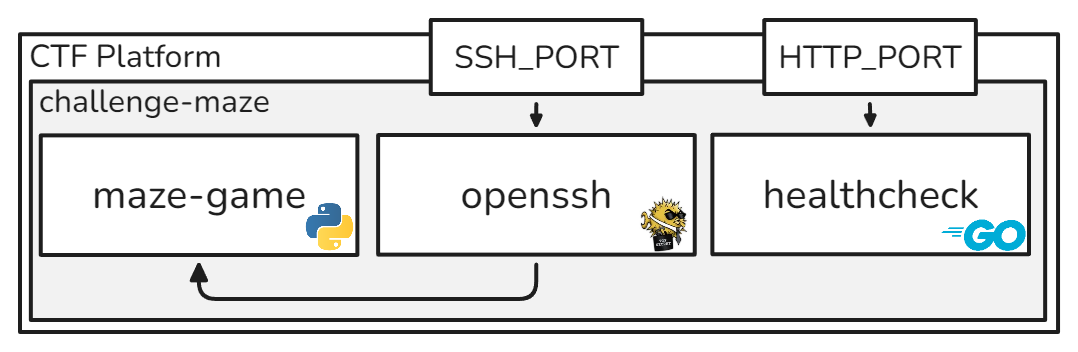
\includegraphics[width=0.85\linewidth]{img/challenge-maze--architecture.png}
    \caption{Maze game challenge architecture}
    \label{fig:maze-architecture}
\end{figure}


\subsubsection{Solution}
Modeling the maze as a graph problem will make it easier to solve. By using the path taken as potential nodes, we can find a solution efficiently. Since the player can backtrack to the start, it is possible to implement BFS. BFS guarantees a solution if one exists, even if the maze has loops and the structure is unknown to the player. Although we don’t have a visible tree or graph, we know our search space, we can then simulate BFS traversal by generating a string like (RbLbRRbRLb...). Here, each 'b' denotes a reset to the start, allowing the player to explore each new path from the beginning. This way, the player explores "R", then "L", then "RR", then "RL", and so on until the solution is found. This BFS string may become very long, so it will be practical to create a script to generate it. The player just needs to find how deep to traverse.



\begin{listing}[H]
  \begin{minted}[linenos]{python}
def BFS(x: int) -> str:
    """generates all possible paths in the given depth in a string 
    >>> BFS(2)
    "RRbLRbRLbLLb"
    """
    last_path = [""]
    i = 0
    while i < x:
        last_path = [y+"R" for y in last_path] + [y+"L" for y in last_path]
        i = i+1
    path = ''.join([y+"b" for y in last_path])
    return path
\end{minted}
  \vspace{-1.5\baselineskip} % Justerer afstanden mellem tekst og liste
 \caption{BFS}
\label{fig:create-account1}
\end{listing}
\noindent
We only need to generate the paths at a given depth. This is an optimization since BFS will explore all previous depths. For example, exploring all nodes at depth five also includes all paths at depths 1-4. So, there is no need to generate paths for previous depths. The number of possible paths (nodes) at depth $h$ is \(2^h\), so generating a BFS traversal string up to depth 50 would result in  \(2^{50}\) paths which each will be 50 characters long followed by a "b", creating an enormous string. This forces us to begin at a reasonable depth and incrementally increase the depth if the solution has not been found to find the solution within a computable space. We can now generate all possible paths. We then only need to insert one character at a time into the maze game to explore all possible paths to find the exit. Since the challenge is hosted on a remote server, accessible via SSH, and the maze game is running at chall:1337, we must first connect to the SSH server to access the game. The code in Appendix \ref{apx:SSHTunnelForwarder_maze} is from the solver and uses an SSH tunnel to forward a local port (127.0.0.1:3242) to the game server's endpoint (chall:1337), which is behind the SSH server. We use the \code{sshtunnel}\cite{sshtunnel} Python package to set up a connection The username and password are provided to the participant (test:test), as well as the host and port of the game service (chall:1337). As shown in Appendix \ref{apx:maze-solver}. We use the pwntools library to automate the process of inserting each character of the generated BFS string into the maze game.
% Note: As input to this function, we will need the given \texttt{REMOTE\_HOST}, \texttt{REMOTE\_PORT} to start the connection.
After the connection is established, we generate a BFS path for a starting depth.
Since the game only accepts one character at once, the script must send each character individually. If the entire path has been sent without finding the solution, the script increases the depth and tries again. This continues until we find the correct path and get the flag.


% know that we can give the the different path strings, like (RL), (RLR), 
% etc.
% Since the solution will be at a depth of 12, the player will need to implement a reasonably optimized solution to generate and test the path string.

% \subsection{Environment and Implementation}

% \subsection{Tools and Resource}

% We are using Python, Docker. The libraries pwntools and sshtunnel is used for the solution.

\subsubsection{Design Choices}

The maze is not a real maze, but rather an acyclic graph where each node has exactly two outgoing edges, one for "left" and one for "right". Where each possible input provided by the player is either "L", "R", or "b", causes the game to traverse the graph accordingly. By designing the graph carefully, we can ensure that there is only one correct path to the exit. The graph contains a single exit node. When the player reaches this node, the game stops and prints a special message, in this case, the flag. This maze implementation, based on a graph, is not a string comparison method. We also thought of two alternative implementations. One would be to use string comparison, and we considered two different ways to approach that. First, we could compare the current path to the correct path that leads to the exit. However, this approach is less efficient because as the path grows longer, the comparison operation becomes more expensive. Alternatively, we could compare the current input character to the expected character in the correct path. This would avoid comparing the full string, but it would still require additional logic to handle situations such as taking a wrong turn or figuring out which character to compare next. Overall, this adds complexity compared to simply traversing the graph and checking whether you've reached the exit node. The graph implementation also makes it easy to design new mazes in the future and adjust their complexity if needed, simply by modifying the maze-graph file without having to change the game files.

 
% \tobias{what does this mean? How is it faster?}

% \esben{Den endelige streng er ikke så lang i dette tilfælde, men hvis den var meget længere, ville problemet være tydeligere. Så ja, i denne labyrint er forskellen måske ikke så stor, men det gælder ikke nødvendigvis for alle labyrinter.

% Hvis man bruger strengsammenligning og sammenligner hele den aktuelle sti med den korrekte sti. Hvis ens nuværende sti er fx 12 tegn lang, kræver det op til 12 sammenligninger for at kontrollere den.

% Tag for eksempel stien rrrrlll. For at nå frem til den skal man først gennemgå r, rr, rrr, rrrr, rrrrl og så videre. Jo længere man bevæger sig, desto længere bliver stien og hver gang man skal sammenligne, skal hele strengen tjekkes fra starten.

% Hvis vi i stedet bruger en graf, som vi burger i challengen.
% Hvis jeg ønsker at følge stien rrrrlll, starter vi i startnoden og bevæger os til dens r-kant. Dette tager konstant tid uanset om det er det første eller det millionte skridt fordi vi kun tager et skridt ad gangen.

% Selvom stien er lang, kræver hvert skridt i grafmetoden ikke, at vi sammenligner hele strengen. Vi foretager blot et hop i grafen. Man kunne måske godt vælge at sammenligne det næste tegn, der gives som input, med det forventede tegn, men i så fald er det stadig nemmere at bruge grafmetoden, da man bare bevæger sig gennem grafen uden at skulle bruge logig til at kontrulere hvor langt man er noget i mazen og om man har lavede en fejl denne logik er ikke nødvendig i gaf metoden.}
% \tobias{Men giver vi ikke kun et input ad gangen? Så skal man vel kun sammenligne med en karakter i strengen, og det er vel det samme som en graf.}
% \esben{hvordan ved man had man skal sammen ligne med?? det behøver vi ikke at vide I gaf metoden men dette skal vi kunne finde I sammenlignings metoden}.
% \tobias{jeg kan bare ikke rigtig se hvorfor det er bedre. Ja vi skal sammenligne direkte med den rigtige sti, men hvorfor er det et problem?}
% \esben{tror jeg er forvigert man kan sammenlige på to måde ended helle ens current path med helle den correct path. ellers skal vi sammen lige en carcter af gangen of så skal vi bruge noget logig til at finde ud af vilken carcter I den recdige path der skal bruget I sammenligningen ja tror heller ikke det er hordiger hvis man sammenliger en carcter af gangen man der skal bruges noget mere logig som ikke er nøvendigt.༼ つ ◕_◕ ༽つ }
% \tobias{hmmmmmmmmmmmmmmm 	⤜(ⱺ ʖ̯ⱺ)⤏  ┌( ͝° ͜ʖ͡°)=ε/̵͇̿̿/’̿’̿ ̿ }

% This grape implementation also simplifies the logic, each move corresponds directly to a transition in the graph. 
% \tobias{I would argue that a string comparison is a whole lot simpler}


The game is essentially endless, since some of the nodes form loops, which means the player can get stuck in an infinite cycle. This makes a naive Depth-First Search ineffective unless it is implemented with a depth limit. The design encourages the player to use Breadth-First Search or a similar strategy to avoid infinite wandering. The decision that the player can only input one character at a time, for example, the player can only move "R", "L", or "b" at any given point in the maze, is intentional. The reason for this design choice is to encourage the player to automate the solution, unless they really want to manually input over 4000+ characters. To play the game, the player must first connect to an SSH server. And when logged in, the player can, for example, use netcat to connect to the maze game running on a specific endpoint. 
% This confession was chosen since It adds a small but meaningful layer of complexity by testing the player's ability to use tools like Pwntools and SSH tunneling, where services are not directly exposed to the public. 

% And it is not possible to have a direct nc (netcat) connection to the CTF platform, so an extra layer, e.g., the SSH server, is necessary for the challenge to work over the internet.

% Initially, we considered that the challenge should establish an SSH connection. However, as we investigated further, we realized that nc (netcat) would have been a good solution for this type of interaction we needed for the challenge. Unfortunately, the CTF platform did not support direct connections via netcat, so we developed a solution that combined both approaches.
% \tobias{I think we talk about this already in the preliminaries}
% \esben{sandt}

By having remote access, the players cannot view the source code of the challenge. This is essential since if these files were exposed, the challenge would be trivial to solve, defeating the purpose of the challenge.




% syndes det lyder lidt blar blar blar skal måske fjernes


\subsubsection{Testing Process}
The first step was to test the core functionality of the maze game, whether the game behaved as expected when receiving input. This was relatively straightforward, since the player is only allowed to input single characters: "r", "l", or "b". We tested all valid and some invalid input scenarios. Examples of invalid inputs include random characters and sequences of valid inputs given as a single line.
% Valid input include (r,v,b,R,V,B). Exampels of invalid inputs include random characters ('g', 'h', 'u', 'a'), and sequences of valid inputs given as a single line ('rr', 'rlrbrl', 'llr', etc.).
As expected, all invalid inputs triggered the game’s help message, which correctly informed the player that the input was not valid. This verified that input validation and feedback worked as intended. The only potential issue we identified is related to how the current path is stored internally in a Python list. If a player continuously inputs a single direction without end (e.g., repeatedly pressing 'r'), the list will grow indefinitely. However, this is not a practical concern, as the number of steps required to exhaust memory on a 64 bit system would require a path length on the order of $2^{63} - 1$ characters\cite{python_maxsize} (Depending on the system's available memory) a scenario that is technically possible but completely unrealistic.

% \tobias{Jeg tror ikke det her er sandt. $2^{63}$ er ca. en 1.000.000.000 GB. Bare fordi addresserne tillader så meget hukkommelse betyder ikke at der er så meget.}
% \esben{kan være jeg ikke forstor men siger vel også (Depending on the system's available memory) ellers også ved jeg ikke hvad du mener :´(  .er det utyligt? Kan godt skrive det om hvis det er}\tobias{maaan i dont hecking know.}

Next, we tested whether the maze was implemented correctly by manually playing the game and verifying that the path to the flag matched the expected result. We then used the BFS based solution file to confirm that the generated path string also successfully reached the flag. Finally, we tested the solver script in three different environments. Locally on our development machine, we built the Docker images, started the challenge, and ran the solver. The solver successfully found and printed the flag. We then tested the solver in a virtual Alpine-based machine. The challenge was deployed, and the solver was run locally. Again, the solver correctly found the flag, and then we tested the challenge using the CTF platform, which once more successfully identified and printed the correct flag. It was successfully verified with challenge ID: \texttt{27260159-69f8-4dbf-8bd9-5ee93f724824}.

% \subsection{Improvements}

% The game could be improved in the following way: it currently prints a lot to the screen when the user provides input, and these write operations are very slow. To optimize this, we could build an entirely new version of the game that isn't text-based, in order to avoid having so many print operations.

\subsubsection{Difficulty Assessment}

% We rate the difficulty as medium. To complete the challenge, the player must:
% Understand breadth-first search. Apply it in a context where the graph is not visible. Know that BFS will find the solution if one exists. Write a script to generate the input string based on BFS traversal and then also generate a script that can input this string into the game, one character at a time, this demands a knowledge of SSH and tools like netcat to have a understanding in how this can be achieved. The challenge becomes significantly more difficult if the player lacks this knowledge.

We rate the difficulty of the challenge as medium. To complete the challenge, the player must first of all understand breadth-first search. Apply it in a context where the graph is not visible. Know that BFS will find the solution if one exists. Write a script to generate the input string based on BFS traversal and then also generate a script that can input this string into the game, one character at a time. This demands knowledge of SSH and tools like \code{pwntools}. The challenge becomes significantly more difficult if the player lacks this knowledge.



